\input{LectureSlides/includes/metropolis_preamble}

% Title page info
\title[Math Review]{Math Review}
\author[ECON 5001]{ECON 5001\\Prof. Healy} \color{metrop}
\institute[OSU]{}
\date[]{\vfill {\tiny Updated \today\ at\ \DTMcurrenttime}}

\begin{document}

\frame{\maketitle}

\begin{frame}{Why a Math Review?}
\begin{itemize}
    \item Official prereqs: ECON 4001.0x and MATH 1151 (Calc 1)
    \item Reality: huge range of experience in the room
    \item Also, some non-calculus concepts
    \item Noting too hard! (IMO)
\end{itemize}
\end{frame}

\begin{frame}{Sets}
    A \textbf{set} is simply a collection of things.
    \begin{itemize}
        \item Example: $A=\{$rock$,$paper$,$scissors$\}$
        \begin{itemize}
            \item Shorthand names: $A=\{r,p,c\}$
        \end{itemize}
        \item Use curly brackets (``braces'')
        \item Comma-separated list
        \item Order doesn't matter
        \item No repetition
    \end{itemize}
    \vfill
    \begin{itemize}
        \item ``Singleton'' set:
        \item Empty set:
    \end{itemize}
\end{frame}

\begin{frame}{Set Operations}
\begin{itemize}
    \item Subset: $A\subseteq B$ and $A\subset B$ \vspace{0.5in}
    \item Union: $A\cup B$ \vspace{0.5in}
    \item Intersection: $A\cap B$ \vspace{0.5in}
    \item Set difference (``set minus''): $A\setminus B$
\end{itemize}
\end{frame}

\begin{frame}{Set Operations}
\begin{itemize}
    \item Universal set: set containing ``all things''  (e.g., possible die rolls)\\(only things we're currently talking about)\vspace{0.6in}
    \item Compl\textbf{e}ment: $A^c=U\setminus A$ \vspace{0.6in}
    \item Element of: $\in$ (and not an element of: $\notin$)\vspace{0.6in}
    \item ``Disjoint'' (mutually exclusive) sets: $A\cap B=\emptyset$
\end{itemize}
\end{frame}

\begin{frame}{Cartesian Product}
The set $S=\{(r,r),(r,p),(r,c),(p,r),(p,p),(p,c),(c,r),(c,p),(c,c)\}$\\ contains \textbf{all possible combinations} of $A=\{r,p,c\}$ and $B=\{r,p,c\}$\\
This is called the \textbf{Cartesian product} (or just \textbf{product}) of $A$ and $B$\\
Notation: $A\times B$.
\bsk
\centering
\begin{tabular}{cc|c|c|c|}
    \cline{3-5}
    & $r$ & \onslide<2>{$(r,r)$} & \onslide<2>{$(p,r)$} & \onslide<2>{$(c,r)$}    \\
    \cline{3-5}
Set $B$ & $p$ & \onslide<2>{$(r,p)$} & \onslide<2>{$(p,p)$} & \onslide<2>{$(c,p)$}    \\
    \cline{3-5}
    & $c$ & \onslide<2>{$(r,c)$} & \onslide<2>{$(p,c)$} & \onslide<2>{$(c,c)$}    \\
    \cline{3-5}
    & \multicolumn{1}{c}{ }  & \multicolumn{1}{c}{$r$} & \multicolumn{1}{c}{$p$} & \multicolumn{1}{c}{$c$} \\
    & \multicolumn{1}{c}{ }  & \multicolumn{3}{c}{Set $A$} \\
\end{tabular}
\vfill
Ren\'{e} Descartes vs. Kazimierz Kuratowski
\vspace{-2in}
\end{frame}

\begin{frame}{Cartesian Product}
You've seen Cartesian products before:
\bsk
\centering
\only<1>{
    \vspace{1.2in}\hspace{-1in}
    \begin{tabular}{cc|c|c|c|}
    \cline{3-5}
    & $r$ & \onslide<1>{$(r,r)$} & \onslide<1>{$(p,r)$} & \onslide<1>{$(c,r)$}    \\
    \cline{3-5}
Set $B$ & $p$ & \onslide<1>{$(r,p)$} & \onslide<1>{$(p,p)$} & \onslide<1>{$(c,p)$}    \\
    \cline{3-5}
    & $c$ & \onslide<1>{$(r,c)$} & \onslide<1>{$(p,c)$} & \onslide<1>{$(c,c)$}    \\
    \cline{3-5}
    & \multicolumn{1}{c}{ }  & \multicolumn{1}{c}{$r$} & \multicolumn{1}{c}{$p$} & \multicolumn{1}{c}{$c$} \\
    & \multicolumn{1}{c}{ }  & \multicolumn{3}{c}{Set $A$} \\
\end{tabular}}\only<2->{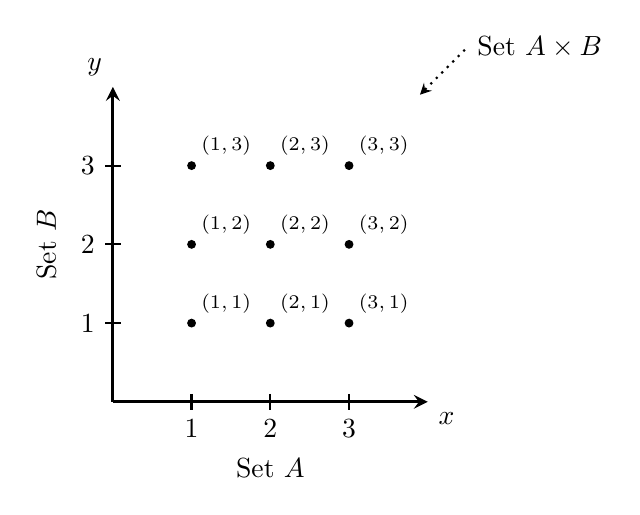
\begin{tikzpicture}[>=stealth]
  % axes
  \draw[line width=1.2pt, ->] (0,0) -- (4,0) node[below right] {$x$};
  \draw[line width=1.2pt, ->] (0,0) -- (0,4) node[above left] {$y$};
  % x-axis ticks and labels
  \foreach \i in {1,2,3}
    \draw[thick] (\i,0.1) -- (\i,-0.1) node[below] {$\i$};
  % y-axis ticks and labels
  \foreach \i in {1,2,3}
    \draw[thick] (0.1,\i) -- (-0.1,\i) node[left] {$\i$};
  \only<3->{
  % axis labels
  \node[below=0.6cm] at (2,0) {Set $A$};
  \node[left=0.6cm, rotate=90, anchor=south] at (0,2) {Set $B$};
  }
  \onslide<4>{  % the 9 points, with labels in small font
  \foreach \x in {1,2,3}
    \foreach \y in {1,2,3} {
      \fill (\x,\y) circle (1.6pt);
      \node[above right=0pt, font=\scriptsize] at (\x,\y) {$(\x,\y)$};
    };
    \draw[line width=0.8pt,dotted, <-] (3.9,3.9) -- (4.5,4.5) node[right] {Set $A\times B$};
    }
\end{tikzpicture}}
    
\end{frame}

\begin{frame}{Indexed Sets}
Sets may be numbered (``indexed''). Example:\\
Player 1's strategies: $S_1=\{a,b\}$\\
Player 2's strategies: $S_2=\{c,d\}$\\
Player 3's strategies: $S_3=\{x,y\}$\\
We can define $S=S_1\times S_2 \times S_3$
\vfill
We can do this for any number $n$ sets: $S=S_1\times S_2\times \cdots \times S_n$\\
Shorthand notation: $S=\times_{i=1}^n\ S_i$
\vspace{-2in}
\end{frame}

\begin{frame}{Lists}
Suppose $S_1=\{r,p,c\}$ and $S_2=\{r,p,c\}$.\\
So $S_1\times S_2=\{(r,r),(r,p),(r,c),(p,r),(p,p),(p,c),(c,r),(c,p),(c,c)\}$.
\bsk
Elements of this set are \textbf{lists}\\
Other names: \textbf{ordered pairs} (if 2), $\bm{n}$-\textbf{tuples} (if $n$), \textbf{vectors}, \uline{\textbf{profiles}}\\
List $(r,c)$ means P1 played Rock and P2 played Scissors
\bsk
Sets vs. Lists:
\begin{center}
\begin{tabular}{c|c|c|}
\cline{2-3}
 & \textbf{Sets} & \textbf{Lists}\\
\cline{2-3}
 & Ex: $\{a,b,c,d\}$ & Ex: $(a,d,d,a)$ \\
\cline{2-3}
 & Braces $\{\cdots\}$ & Parentheses $(\cdots)$  \\
\cline{2-3}
 & Comma-separated & Comma-separated \\
\cline{2-3}
 & Order doesn't matter & Order matters!!! \\
\cline{2-3}
 & Cannot repeat & Can repeat \\
\cline{2-3}
\end{tabular}
\end{center}
Confusing: $(0,10)$ can represent a list or an interval.
\end{frame}

\begin{frame}{Cartesian Products \& Lists}
    Rock-Paper-Scissors:\\
    $S_1=\{r,p,c\}$\\
    $S_2=\{r,p,c\}$\\
    $S=S_1\times S_2$ (Cartesian product)\\
    $S=\{(r,r),(r,p),(r,c),(p,r),(p,p),(p,c),(c,r),(c,p),(c,c)\}$\\
    Each element of $S$ is a \textbf{list}\vspace{0.5in}
    
    List says (1) what P1 chose in $S_1$, (2) what P2 chose in $S_2$ 
    \vfill
    In game theory, lists of strategies are \textbf{strategy profiles}. e.g. $(r,c)$.
    \vspace{-1in}
\end{frame}

\begin{frame}{Strategy Profiles With $n$ Players}
Game theory notation:
\begin{itemize}
    \item Suppose a game has $n$ players
    \item What does this mean: ``Each player $i$ chooses some $s_i\in S_i$''
    \item Any particular player number:\hspace{0.5in} $i\in \{1,2,\ldots,n\}$
    \item Set of possible strategies for player $i$:\hspace{0.1in} $S_i$
    \item A particular strategy for player $i$:\hspace{0.42in} $s_i$
\end{itemize}
Player 1 chooses $s_1\in S_1$\\
Player 2 chooses $s_2\in S_2$\\
$\vdots$\\
Player $n$ chooses $s_n\in S_n$
\bsk
Strategy profile $s=(s_1,s_2,\ldots,s_n)\in S=S_1\times S_2\times \cdots S_n$
\end{frame}

\begin{frame}{``Not $i$'' Notation: $s_{-i}$}
\begin{itemize}
    \item Suppose there are $n$ players
    \item Each player $i$ plays strategy $s_i$
    \item The profile is $s=(s_1,s_2,s_3,\ldots,s_n)$
    \item Suppose we want to focus on player 7
    \begin{itemize}
        \item ``I am player 7'', so set $i=7$
    \end{itemize}
    \item In this case, $i=7$. So $s_i=s_7$
    \item The strategies of others are $s_{-7}=(s_1,s_2,\ldots,s_6,s_8,\ldots,s_n)$
    \item For any player $i$, call this $s_{-i}$
    \begin{itemize}
        \item $s_{-7}=(s_1,s_2,\ldots,s_6,s_8,\ldots,s_n)$
        \item $s_{-3}=(s_1,s_2,s_4,\ldots,s_n)$
        \item $s_{-1}=(s_2,s_3,\ldots,s_n)$
    \end{itemize}
    \item The entire profile can be written as $s=(s_i,s_{-i})$
    \begin{itemize}
        \item $s_i$ is what player $i$ plays
        \item $s_{-i}$ is what all the other players play
    \end{itemize}
\end{itemize}
    
\end{frame}

\begin{frame}{Functions}
    Function you're probably used to: $y=x^2$ or $f(x)=x^2$
    \vspace{1in}
    
    What is this function doing? Mapping one set into another!
    \vfill
    Domain vs. Range (or ``Codomain'')
    \vspace{-1.5in}
    
\end{frame}


\begin{frame}{More General Functions}
Any domain and any range. Ex: classes of animals.
\tikzset{
  item/.style={
    draw, rounded corners=2pt, fill=white,
    minimum width=2.9cm, minimum height=0.56cm,
    font=\sffamily\small, inner sep=2pt, anchor=center
  },
  classitem/.style={item, fill=blue!8,   draw=blue!55,   very thick},
  speciesitem/.style={item, fill=orange!10, draw=orange!70, very thick},
  setlabel/.style={font=\sffamily\bfseries},
  caption/.style={font=\sffamily\itshape\scriptsize, text=black!60},
  maparrow/.style={-{Stealth[length=2.6mm]}, line width=0.8pt, draw=black!65}
}
\centering
\begin{tikzpicture}
  \node[speciesitem] (d1) {Axolotl};
  \node[speciesitem, below=0.22cm of d1] (d2) {Platypus};
  \node[speciesitem, below=0.22cm of d2] (d3) {Komodo dragon};
  \node[speciesitem, below=0.22cm of d3] (d4) {Coelacanth};
  \node[speciesitem, below=0.22cm of d4] (d5) {Kiwi};
  \node[speciesitem, below=0.22cm of d5] (d6) {Pangolin};
  \node[speciesitem, below=0.22cm of d6] (d7) {Hammerhead shark};
  \node[speciesitem, below=0.22cm of d7] (d8) {Hoatzin};
  % ---- range (classes): right column --------------------------------
  \node[classitem, right=4.2cm of d2, yshift=0cm] (r1) {Fish};
  \node[classitem, below=0.48cm of r1] (r2) {Amphibians};
  \node[classitem, below=0.48cm of r2] (r3) {Reptiles};
  \node[classitem, below=0.48cm of r3] (r4) {Birds};
  \node[classitem, below=0.48cm of r4] (r5) {Mammals};

  % ---- set labels ---------------------------------------------------
  \node[setlabel] (dlab) at ($(d1.north)+(0,0.6)$) {Domain};
  %\node[caption, below=0pt of dlab] {animals};
  \node[setlabel] (rlab) at (dlab -| r1) {Range};
  %\node[caption, below=0pt of rlab] {classes};

  % ---- enclosing sets ----------------------------------------------
  \begin{scope}[on background layer]
    \node[draw=orange!70, very thick, rounded corners=12pt,
          fit=(d1)(d8), inner sep=8pt, fill=orange!4] {};
    \node[draw=blue!55, very thick, rounded corners=12pt,
          fit=(r1)(r5), inner sep=10pt, fill=blue!4] {};
  \end{scope}

  % ---- the mapping: appears on overlay 2 ----------------------------
  \only<2->{
    \draw[maparrow] (d1.east) -- (r2.west); % Axolotl          -> Amphibians
    \draw[maparrow] (d2.east) -- (r5.west); % Platypus         -> Mammals
    \draw[maparrow] (d3.east) -- (r3.west); % Komodo dragon    -> Reptiles
    \draw[maparrow] (d4.east) -- (r1.west); % Coelacanth       -> Fish
    \draw[maparrow] (d5.east) -- (r4.west); % Kiwi             -> Birds
    \draw[maparrow] (d6.east) -- (r5.west); % Pangolin         -> Mammals
    \draw[maparrow] (d7.east) -- (r1.west); % Hammerhead shark -> Fish
    \draw[maparrow] (d8.east) -- (r4.west); % Hoatzin          -> Birds
  }
\end{tikzpicture}
\end{frame}

\begin{frame}[t, plain]{A Game Theory Example}
\textbf{Rock-Paper-Scissors:}\\
9 possible strategy pairs: $S=\left\{\begin{tabular}{ccc}
(r,r),&(r,p),&(r,c),\\
(p,r),&(p,p),&(p,c),\\
(c,r),&(c,p),&(c,c)
\end{tabular}\right\}$\\
First letter: P1's choice. Second letter: P2's choice\\
Outcomes: $O=\{$P1Wins$,$Tie$,$P2Wins$\}$
\par\vfill
``Outcome function''
\vspace{-1.75in}
\end{frame}

\begin{frame}{A Game Theory Example}
    We can represent this in table format.\\
    \textbf{Convention:} Player 1 is rows, Player 2 is columns
    \bsk
    \centering
    \begin{tabular}{ccc}
        Strategy pairs: & & Outcome function: \\
         & & \\
        \begin{tabular}{cc|c|c|c|}
            & \multicolumn{1}{c}{ }  & \multicolumn{3}{c}{Set $S_2$} \\
            & \multicolumn{1}{c}{ }  & \multicolumn{1}{c}{$r$} & \multicolumn{1}{c}{$p$} & \multicolumn{1}{c}{$c$} \\
            \cline{3-5}
            & $r$ & \onslide<1->{$(r,r)$} & \onslide<1->{$(r,p)$} & \onslide<1->{$(r,c)$}    \\
            \cline{3-5}
            Set $S_1$ & $p$ & \onslide<1->{$(p,r)$} & \onslide<1->{$(p,p)$} & \onslide<1->{$(p,c)$}    \\
            \cline{3-5}
            & $c$ & \onslide<1->{$(c,r)$} & \onslide<1->{$(c,p)$} & \onslide<1->{$(c,c)$}    \\
            \cline{3-5}
        \end{tabular} 
        & $\rightarrow$ &
        \begin{tabular}{c|c|c|c|}
            \multicolumn{4}{c}{ }\\
            \multicolumn{1}{c}{ }& \multicolumn{1}{c}{$r$} & \multicolumn{1}{c}{$p$} & \multicolumn{1}{c}{$c$} \\
            \cline{2-4}
            $r$ & \onslide<2>{Tie} & \onslide<2>{P2} & \onslide<2>{P1}    \\
            \cline{2-4}
            $p$ & \onslide<2>{P1} & \onslide<2>{Tie} & \onslide<2>{P2}    \\
            \cline{2-4}
            $c$ & \onslide<2>{P2} & \onslide<2>{P1} & \onslide<2>{Tie}    \\
            \cline{2-4}
        \end{tabular} 
    \end{tabular}
\end{frame}

\begin{frame}{A Bit of Calculus}
Set of all ``real'' numbers: $\Bbb{R}=(-\infty,\infty)$ (interval)\\
``Real'' function: domain and range are both $\Bbb{R}$
\bsk
\centering
\begin{tikzpicture}[>=stealth,scale=0.8]
  % axes
  \draw[line width=1.2pt, <->] (-0.9,0) -- node[below]{} (8,0) node[below right] {$x$};
  \draw[line width=1.2pt, <->] (0,-0.9) -- node[left]{} (0,6) node[above left] {$y$};

  \draw[line width=0.8pt,dotted, <-] (8,5) -- (9,6) node[right] {Set $\Bbb{R}\times \Bbb{R}$};
%  \draw[blue, thick, smooth, samples=100, domain=0:5]    plot (\x, {(\x-3)*(\x-3)*(\x-3) - 3.5*(\x-3) + 3});
\end{tikzpicture}
\end{frame}

\begin{frame}{A Bit of Calculus}
    \only<1>{What is the slope at a point?}
    \only<2>{What is the derivative?}
    
\begin{tikzpicture}[>=stealth,scale=0.8]
  % axes
  \draw[line width=1.2pt, <->] (-0.9,4) -- node[below]{} (8,4) node[below] {$x$};
  \draw[line width=1.2pt, <->] (0,3.5) -- node[left]{} (0,7) node[left] {$y$};
%  \draw[blue, thick, smooth, samples=100, domain=0:5]    plot (\x, {(\x-3)*(\x-3)*(\x-3) - 3.5*(\x-3) + 3});
  \draw[line width=1.2pt, <->] (-0.9,0) -- node[below]{} (8,0) node[below] {$x$};
  \draw[line width=1.2pt, <->] (0,-0.9) -- node[left]{} (0,3) node[left] {$y$};
\end{tikzpicture}
\end{frame}

\begin{frame}{A Bit of Calculus}
    How to find the max of a function using calculus?

    \begin{tikzpicture}[>=stealth,scale=0.8]
      % axes
      \draw[line width=1.2pt, <->] (-0.9,4) -- node[below]{} (8,4) node[below] {$x$};
      \draw[line width=1.2pt, <->] (0,3.5) -- node[left]{} (0,7) node[left] {$y$};
    %  \draw[blue, thick, smooth, samples=100, domain=0:5]    plot (\x, {(\x-3)*(\x-3)*(\x-3) - 3.5*(\x-3) + 3});
      \draw[line width=1.2pt, <->] (-0.9,0) -- node[below]{} (8,0) node[below] {$x$};
      \draw[line width=1.2pt, <->] (0,-0.9) -- node[left]{} (0,3) node[left] {$y$};
    \end{tikzpicture}
\end{frame}

\begin{frame}{A Bit of Calculus}
    A worked example.
    \begin{itemize}
        \item Function: $f(x) = 4+2x-6x^2$
        \item Derivative: $f'(x) =$
        \item Set equal to zero: 
        \item Solve: 
    \end{itemize}
      \begin{tikzpicture}[>=stealth,scale=0.8]
      % axes
      \draw[line width=1.2pt, <->] (-1,0) -- node[below]{} (5,0) node[below] {$x$};
      \draw[line width=1.2pt, <->] (0,-1) -- node[left]{} (0,4) node[left] {$y$};
      \draw[blue, thick, smooth, samples=100, domain=0:5]    plot (\x, {4+2*(\x)-6*(\x)*(\x)});
    \end{tikzpicture}
\end{frame}
\end{document}
